\documentclass[12pt,french,english,notitlepage]{report} % main lang last
%\documentclass[12pt,english, spanish, french]{thesis}
%
% usage notes: 
% - Place figures in the /fig folder
% - Place chapters in the /chapters folder.
% - References should be included in ./mybib.bib


% Some page styling:
%\usepackage[a4paper,width=150mm,top=25mm,bottom=25mm]{geometry}
\usepackage[margin=0.7in]{geometry}
%\usepackage{fancyhdr}
%\pagestyle{fancy}

\usepackage[utf8]{inputenc}
\usepackage[english]{babel}
\usepackage{caption}
\usepackage{subcaption}
% Interlineado
%\usepackage{setspace}
%\setstretch{1.5}

% Bibtex
%\usepackage{cite} % use cite with natbib but not with biblatex
%\usepackage{natbib}
\usepackage[style=numeric,backend=bibtex]{biblatex}
\bibliography{refs} % put here in preamble when using biblatex

\usepackage[titletoc]{appendix}
\usepackage{float}
\usepackage{graphicx}
\usepackage{rotating}
%\usepackage{eso-pic}
%\usepackage{multicol}
\usepackage{enumerate} % custom lists
%\usepackage{url}
%\usepackage{soul}
% for working with eps
\usepackage{epstopdf} 
\usepackage{color} % color text
\usepackage{titlesec} % to change the way \paragraph formats the titles
\usepackage{textcomp} % for copyright symbol
\usepackage{quotchap} % for chapter openning quotes
\usepackage{titling}
\usepackage{tablefootnote}

% Define a path for the fig folder
% nota: imges must be in the same folder or subfolders of this file, if not pdf2latex will complain
% ---------------------- %
\newcommand{\figpath}{./fig}
%\graphicspath{ {./fig/} }

% Bibligraphy path
% ---------------------- %
\newcommand{\bibpath}{.}

\usepackage[hidelinks]{hyperref}

% ---------------------- %
% Title
% ---------------------- %
\title{The Legacy Project}
\author{
  Michel, Nicolas\\
  \texttt{nicolas@legacy.network}
  \and
  Almonacid, Vicente\\
  \texttt{vicente@legacy.network}
}
\date{\today\\v0.7}

% end preamble
%

% Start content
% -------------------------------------------------------------------------------------- %
\begin{document}

% \begin{titlingpage}
%     \maketitle
%     \begin{abstract}
%         Legacy is a blockchain-based application that allows people to easily distribute assets upon their dead (or, in general, upon any verifiable event).
%     \end{abstract}
% \end{titlingpage}

\maketitle
\begin{abstract}
    Legacy is a blockchain-based application allowing people to easily distribute assets upon their death or, in general, upon any set of verifiable events.
    The application integrates a variety of services that will be developed progressively as blockchain technology consolidates. 
    This paper mainly describes Legacy's initial releases, which allow to transfer digital assets, such as images, videos and text documents. 
    The application core functionalities will be initially developed on the Ethereum blockchain. These include a Proof of Life engine responsible of determining whether the user is alive or not, and a smart contract that manages user assets and schedules their distribution according to a given set of triggering events.
    Exploiting the unique characteristics of blockchain platforms, Legacy is designed in order to ensure security, reliability and long-term availability. 
    Typical use cases include transfer of sensible data (\textit{e.g.}, personal meaningful data), cryptocurrency holdings and confidential data such as online service account credentials.
    In the long-term, Legacy expects to integrate smart property and other blockchain-based digital assets, as well as to provide a platform for peer-to-peer legal and technical assistance, thus becoming a next-generation smart-will solution.

\end{abstract}


% acknowledgements
\chapter*{Acknowledgements}

The Legacy Project wouldn't have been possible without the desinterested support and valuable feedback from many individuals.
Directly or indirectly, they have also helped us to improve this document significantly.
We would like to express our deep gratitude to (without any particular order):
Laurent Hardy from Madrid's Ethereum Community, Marina Markežič from Cofoundit, Arturs Zelenkovecs, Scott Stevenson, Benoît Belin, reddit users FjorXD and rpr11; Aragon team members Jorge, Luis and tatu; Virginie Gretz, Sebastien Bourguignon, Phillipe Rodriguez, Adrian Brink, Roman Beyon from La Maison du Bitcoin and CTO of iExec Oleg Lodygensky.

% to confirm:  Kevin Sahin, Nacer Laradji, Philippe Dardier,



\tableofcontents

% \listoffigures

% ---------------------- %
% Main Content
% ---------------------- %

\chapter{Executive Summary} % (fold)
\label{cha:executive_summary}

Wills, or testaments, have a history that goes back to Ancient Greece. While their utility and legal implications contrast among different cultures and ages, their underlying mechanisms are basically the same. As we move toward a digital economy and society, analog forms of value---including both sentimental and monetary--are being replaced, stored and transmitted in digital formats. In this way, printed documents, books, pictures---and even money--are just a few examples of things that are now regularly handled digitally. In this context, distributing our valuable digital possessions after we pass away is not something that can be easily achieved through the traditional system consisting of a simple Will and an executor. In particular, this approach usually requires the intervention of several trusted third parties (an executor, a lawyer and eventually a public notary) and does not guarantee security, reliability nor privacy--the latter being especially important when it comes to transferring personal data to which we attribute profound meaning. Furthermore, with the introduction of blockchain platforms and smart contracts, on the one hand, and the imminent mainstream adoption of the Internet of Things (IoT), on the other, we expect to see the emergence of a novel concept of property known as \textit{smart property}; that is, a type of property that can be traded and transferred without the need for intermediaries. Just as cryptocurrencies, smart property will require a different technological solution--as well as a novel legal framework--in order to be securely transferred according to a decedent last Will.
This paper introduces Legacy, a blockchain-based service that aims at becoming the first \textit{smart Will}. At a first stage, Legacy will focus on providing a service allowing you to distribute what we refer to as \textit{memories}; \textit{i.e.}, digital items such as images, video recordings, songs, manuscripts or other forms of digital data that captures essential life experiences or holds significant sentimental value. In the long term, as smart property becomes a reality and law embraces the blockchain revolution, Legacy aims at positioning as the \textit{de facto} smart will solution, progressively eliminating the need for trusted third parties and ensuring key attributes such as security, privacy and long-term operation.

% ---------------------------------------------------------------------------------------------------------------- %
% Problem Statement
% ---------------------------------------------------------------------------------------------------------------- %
\section{Problem Statement} % (fold)
\label{sec:problem_statement}
The traditional process of transferring property---whether it be in the form of real estate, money or ordinary valuable objects---through a will and testament involves several issues, which vary depending on the particular legal framework. 

In general, the process depends entirely on an executor, who is in charge of administrating the legacy and is appointed by the testator (i.e., the person who writes the will). An executor should therefore be someone in whom the testator absolutely trust.  Writing a conventional will might also require the intervention of additional  intermediaries, such as a lawyer and a notary. In many cases, however, these are not legally indispensable, which suggests that the process can be systematized in order to be easily self-completed by the testators. The OpenLaw protocol recently proposed by Consensys \cite{cite_required} is an interesting innovation on this subject. 

Wills are typically written in the form of simple, ordinary documents, and hence can get lost or destroyed. Since they must be easily accessible by the executors when the moment arrives, wills are usually not stored securely. This also compromises the integrity and confidentiality of the content.
  
Conventional wills are in general limited to the distribution of monetary valuable possessions and are not suitable for managing personal digital data. Nowadays, most of our important life experiences and memories are captured in emails, digital images, videos,  and other forms of digital items. All of these are also part of our legacy and require  and, naturally, conventional wills are not meant to this purpose. While software solutions addressing this problem exist, these are in general based on centralized solutions that provide limited guarantees in terms of reliability and long-term operation.

A conventional will is defined and executed once. Making further modifications after it has been signed is in general not possible and requires rewriting the entire document. A will is also inherently static in the sense that it cannot be automatically adapted according to changes in future conditions or unpredictable events. In addition, the process of executing a will may take significant time. Much of the process can be accelerated and systematized by taking advantage of simple software solutions. 

Finally, there is the problem of securely transferring cryptocurrencies. Currently, cryptocurrencies are stored in wallets that can be accessed through a private key or password-protected encrypted files. If an individual holding cryptocurrencies dies without having communicated his/her wallet credentials to third persons, then the entire wallet balances are irrevocably lost. 

% section problem_statement (end)

% ---------------------------------------------------------------------------------------------------------------- %
% Goals
% ---------------------------------------------------------------------------------------------------------------- %
\section{Goals} % (fold)
\label{sec:goals}

\subsubsection*{Simplifying the process of transferring your digital possessions after your death} % (fold)
\label{ssub:simplifying_the_process_of_transferring_your_digital_possessions_after_your_death}
Legacy is an easy-to-use application that aims at removing the burden of dealing with multiple services. Exploiting the advantages blockchain-based smart contracts, Legacy allows to transfer digital data without relying on an trusted intermediary.  
Through the Legacy web interface or mobile application, a user can easily select who---and under which conditions---will receive what when the time come.
% subsubsection simplifying_the_process_of_transferring_your_digital_possessions_after_your_death (end)

\subsubsection*{A service that ensures security, reliability, privacy and long-term operation} % (fold)
\label{ssub:a_service_that_ensures_security_reliability_privacy_and_long_term_operation}
Today, anyone can host files on the cloud and call it secure. Legacy goes beyond and above, with public, auditable code. Hosting code and critical data in the Ethereum Blockchain also ensures its availability in the future. In addition, a system design approach oriented towards decentralization allow us to increase the service reliability.
We are committed to building a system that is provably honest---and one that will outlive both us and our company.
% subsubsection a_service_that_ensures_security_reliability_privacy_and_long_term_operation (end)

\subsubsection*{Reducing the need for trusted third parties for creating and executing a will} % (fold)
\label{ssub:reducing_the_need_for_trusted_third_parties_for_creating_and_executing_a_will}
The need for trusted third parties for transferring property usually has more to do with legal issues rather than technical requirements. In this context, advanced algorithms combined with smart contracts allow to simplify the process.
% subsubsection reducing_the_need_for_trusted_third_parties_for_creating_and_executing_a_will (end)

\subsubsection*{An enhanced, smart will allowing to transfer cryptocurrency and smart property} % (fold)
\label{ssub:_an_enhanced_smart_will_allowing_to_transfer_cryptocurrency_and_smart_property_}
Our ultimate goal is to integrate a wide variety of transferable items, including cryptocurrencies and other types of virtual assets, as well as smart property. This the long-term vision of the Legacy project and represents the main problems that we aim to tackle. This goal, however, involves a number of technical challenges and legal issues that need to be overcome---as we discuss in more detail later on.
% subsubsection _an_enhanced_smart_will_allowing_to_transfer_cryptocurrency_and_smart_property_ (end)

% section goals (end)

% ---------------------------------------------------------------------------------------------------------------- %
% Overview of Legacy and Use Cases
% ---------------------------------------------------------------------------------------------------------------- %
\section{Overview of Legacy and Use Cases} % (fold)
\label{sec:overview_of_legacy_and_use_cases}
In the mid term, the Legacy project is divided into two main phases, as detailed in Section \ref{roadmap_section}: Legacy I and Legacy II---the main differences between both being in the underlying software architecture.  Further releases including enhanced capabilities---such as the ability to manage smart property---are also considered over the medium and long terms, as technological and legal issues are overcome. This document focuses mainly on Legacy I and II, which we will refer to simply as Legacy in the following. 

Initially, Legacy will allow to securely transfer any form of digital data such as pictures, videos, audio files and text documents. Files will be stored using a decentralized, encrypted system. Each individual file belonging to a given user represents a memory. Memories can be bundled into capsules that a user may schedule for transfer to one or more recipients upon death. A capsule can be programmed in many different ways, forming a smart will. For instance, a user might want to send an email to his/her children once they turn eighteen years old or share with them special memories for important days of their lives such as graduation or marriage. In this way, a user can easily specify which are the events and conditions that trigger a capsule transfer.

An important function of the Legacy application is to determine precisely and timely whether the user is alive or not---ideally without involving interaction with family members. This is verified periodically through a mechanism called Proof of Life (PoL). The PoL engine uses different criteria in order to take a reliable decision, and its operation can be completely customizable by the user. For instance, PoL can be based on social network activity patterns---which has the advantage of not requiring explicit signalling from the user---or on periodic email notifications asking the user to simply click on a link. Different PoL mechanisms can be combined in order to achieve a desired level of reliability and user experience. Once the PoL engine determines that the user has died, the capsules are scheduled for further distribution.

\subsection{Cryptocurrencies and Smart-property: The Legacy Vision} % (fold)
\label{sub:cryptocurrencies_and_smart_property_the_legacy_vision}
With the introduction of blockchain technologies and smart contracts, as well as the global deployment of the IoT, the concept of smart property will rapidly become a reality.  At this stage, the challenges are no longer technological, but legal. The same applies for cryptocurrencies. Legacy will study applicable legislation in our customers countries, and spearhead the transition to smart property by providing a clear reference framework. 
% subsection cryptocurrencies_and_smart_property_the_legacy_vision (end)

% section overview_of_legacy_and_use_cases (end)



% chapter executive_summary (end)
%\chapter{Business Model} % (fold)
\label{cha:business_model}


% ---------------------------------------------------------------------------------------------------------------- %
% Market Potential
% ---------------------------------------------------------------------------------------------------------------- %
\section{Market Potential and Customer Segments} % (fold)
\label{sec:markt_potential_and_customer_segments}
Most of Legacy’s customers are expected to fit one of the following categories:
\begin{itemize}
	\item People in their mid-thirties, who are moving in with a significant other or having kids. They are experiencing the first memories of building their own family, and want to preserve them.
	\item Baby boomers and seniors: people who start planning the last stage of their lives and/or those suffering illness. They feel at the end of their journey, and want to share what they learned and experienced.
	\item Professionals in a high-risk environment, such as firefighters, loggers, fishermen, etc.
	\item People needing a proven “dead man switch” to distribute documents.
\end{itemize}

Legacy is oriented to the average Internet user. We put special focus on seniors  and baby boomers, as this public might feel particularly concerned with the problems that Legacy aims to solve. As a result, the Legacy interface is designed in order to be simple and intuitive. In principle, since both Memoirs and Heritage releases should not involve major legal issues, access to the global market is envisaged. Future releases including enhanced capabilities (i.e., cryptocurrencies, smart property) throughout different countries will require a case-to-case study regarding the specificities of each local regulation and will be deployed progressively. Particular attention (in terms of language, legal and customer support) will be given to markets where the demand for next-generation digital services is potentially higher, i.e., the European, Asian and North American markets. Business expansion to other regions is foreseen at a later stage, according to the observed demand.  

The rapid growth of the overall cryptocurrency market capitalisation has also given rise to another significant market segment. As mentioned above, holders of cryptocurrency currently lack of a reliable mechanism to secure their holdings in case of decease. Legacy is the first platform aiming at tackling this issue. Similarly, smart property will require reliable transfer and distribution mechanisms, which brings additional market opportunities. 

% section markt_potential_and_customer_segments (end)

% ---------------------------------------------------------------------------------------------------------------- %
% Competitive Analysis
% ---------------------------------------------------------------------------------------------------------------- %
\section{Competitive Analysis and Unfair Advantage} % (fold)
\label{sec:competitive_analysis_and_unfair_advantage}

Several competitors claim to offer a product similar to Legacy (see for instance \url{legacyvault.com} and \url{knotify.me}). Most of these services, however, are based on a centralized structure, making their customers vulnerable to a single point of failure: the company hosting the service. Some cited examples in the appendix show some that have already closed at the time of writing this document.

Most of the competitors also rely on an annual billing cycle, making the service total price an unknown quantity. By contrast, Legacy offers a one-time payment option, offering the peace of mind that memories will not be lost should the customer suffer hardship in his future.

Two examples that are exceptions in our competition analysis are lastwill.io and digipulse.io, both of which, to some extent, are blockchain based services. But both have a limited view of what the smart will can do, and mainly target cryptocurrency owners, which we believe is a mistake in the market analysis.

The durable, auditable, and transparent nature of Legacy, detailed below, places it in a category of its own.

% ---------------------------------------------------------------------------------------------------------------- %
% Service Operation
% ---------------------------------------------------------------------------------------------------------------- %
\section{Service Operation, Fees and Revenue} % (fold)
\label{sec:service_operation_fees_and_revenue}
Legacy users are able to sign-up to the application for free. A free account allows to explore the application interface, upload files (memories) and organize them into capsules. A subscription is required in order to commit a capsule. From a technical point of view, committing a capsule results in the creation of a smart contract on the blockchain and the initiation of the PoL engine, which involves transaction and operational fees. Subscripted users also benefit from a secure, decentralized file storage system.

Several subscription packages will be proposed. These differ according to the amount of storage capacity, PoL reliability level and additional services such as special customer support, including legal advice or access to professional storytelling specialists.

Subscription fees will be charged on a lifetime or periodic basis, and can be paid through fiat currencies as well as through conventional cryptocurrencies such as ether. In addition, subscription fees may be paid through the Legacy token, which provides users with commercial advantages.

The target price of the lifetime Legacy subscription is between 250€ and 500€.
% section service_operation_fees_and_revenue (end)

% ---------------------------------------------------------------------------------------------------------------- %
% Customer Relations
% ---------------------------------------------------------------------------------------------------------------- %
\section{Customer Relations and Channels} % (fold)
\label{sec:customer_relations_and_channels}
Convincing user to entrust their memories to Legacy implies building long-term confidence in our product.
For all segments, marketing campaigns will be carried mainly on the web in order to bring potential customers to the website where they can sign-up.
Legacy will also partner with players in specific markets, such as life insurance providers. The Legacy service can be bundled in global offers, in particular from established players in the Silver Economy.
The most costly part of the customer relationship will be providing tailored legal advice to specific customers: this will be part of a premium package.

In all cases, Legacy will provide powerful onboarding tools to make the experience as simple as possible, such as automatically building capsules and contacts based on social network activity.
% section customer_relations_and_channels (end)

% ---------------------------------------------------------------------------------------------------------------- %
% Cost Structure
% ---------------------------------------------------------------------------------------------------------------- %
\section{Cost Structure} % (fold)
\label{sec:cost_structure}
Most of Legacy’s costs will come from the team salaries. For details, see Section \ref{Resource Allocation}.
Each customer will also have a recurring cost for Proof of Life verification. We estimate the average customer to be around 48 years old. Taking into account a life expectancy of 80 years, the average service duration for a customer is calculated at 32 years.

Using the estimates outlined in this section, Legacy will become profitable in 2022, with 8 million USD needed in funding to reach that goal.

\begin{figure}[h]
  \centering
  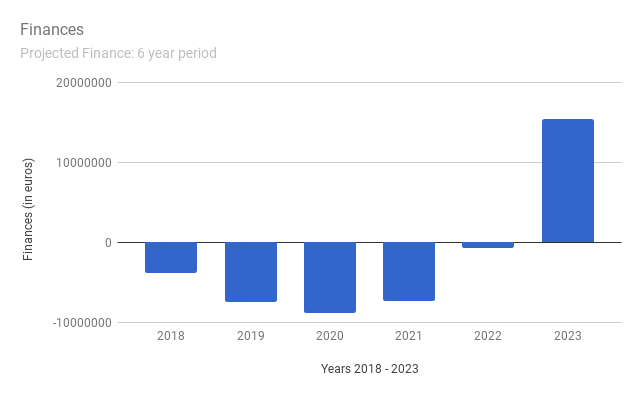
\includegraphics[scale=0.5]{fig/finances_chart}
  \caption{Projected finances: 6-year time span.}
  \label{fig:projected_finances}
\end{figure} 

% section cost_structure (end)

% chapter business_model (end)
\chapter{Implementation} % (fold)
\label{cha:implementation}

% TO-DO
This chapter focuses on software implementation aspects and related issues. We identify key attributes that Legacy must exhibit and describe the adopted approaches to tackle them. Overall, Legacy’s underlying implementation aims at building a robust application that inspires confidence from both users and investors.

As mentionned, Legacy’s core functionalities reside in the Ethereum blockchain platform \cite{Ethereum}. This aspect is perhaps the main competitive advantage of Legacy with respect to similar solutions, and also enables additional functionalities that have not been addressed by other services. 
%Before introducing Legacy’s general architecture, the reasons why a blockchain platform has been adopted are briefly discussed next.

% ---------------------------------------------------------------------------------------------------------------- %
% Why Blockchain
% ---------------------------------------------------------------------------------------------------------------- %
\section{Why Blockchain?} % (fold)
\label{sec:why_blockchain_}

The essential role of a blockchain consists on removing the dependency on trusted third parties in networks where nodes are non-reliable. In this way, any pair of nodes may exchange and process data securely without the intervention of intermediaries. In this way, Bitcoin eliminated the requirement for banks as validators of money transactions. The introduction of smart contracts has paved the way for many novel blockchain applications. Basically, smart contracts not only allow to securely perform peer-to-peer money transactions, but virtually any type of operation. In addition, smart contracts can be executed programmatically and in response to real world events (i.e., events outside of the blockchain). In our context, a blockchain platform supporting smart contracts also allows us to guarantee the main following properties: 

\begin{itemize}
	\item Authenticity: a will stored in the form of a smart contract allows to fully guarantee that all its content was actually dictated by its original author.
	\item Immutability: once a smart contract has been signed and uploaded to the blockchain, it cannot be modified nor deleted by attackers.
	\item Reliability: most blockchains consists of a large number of nodes that jointly validate the current system state. Smart contract data and transaction records are safely stored, validated and replicated at each network node. Hence, It is very difficult for an attacker to disrupt the network or corrupt the data.
\end{itemize}

% section why_blockchain_ (end)

% ---------------------------------------------------------------------------------------------------------------- %
% Technical Aspects
% ---------------------------------------------------------------------------------------------------------------- %
\section{Technical Aspects} % (fold)
\label{sec:technical_aspects}

\subsection{Data Storage} % (fold)
\label{sub:data_storage}
Using Ethereum smart contracts guarantees that the code is reliably stored and that user's dispositions, as specified in the contract, remain immutable in the long term (unless, of course, they are modified by the user himself). However, storing data directly on the blockchain is currently prohibitively expensive.
For instance, an SSTORE operation, which stores a 256-bit word on the Ethereum blockchain, costs 20000 gas \cite[Appendix G]{Wood}. Hence, storing 1 Gigabyte of data on the Ethereum blockchain would cost around 13000 ETH, or, equivalently, about 4 million USD\footnote{At the moment of writing these lines gas price is 21 Gwei and 1 ETH $\equiv$ 250 EUR.}.
In fact, due to the amount of overhead involved, blockchains are not designed for data storage, which is why it is disincentivized by imposing fees. 

As a consequence, data storage requires a different approach. Currently, several alternatives are being discussed and investigated by the Legacy team.
Among some identified third-party providers we may mention:

\begin{itemize}
	\item Swarm
	\item Usenet
	\item Storj
	\item Sia
	\item Filecoin
\end{itemize}

These are all based on decentralized architectures and have been considered as candidate solutions for Legacy.
In partiular, blockchain-based file storage provides high reliability, DDOS resistance, fault tolerance, among other desirable attributes. 

To further improve storage reliability, more ``traditional'' services can be also considered, as for instance local storage (\textit{i.e.}, using Legacy's infrastructure), Glacier by Amazon, hubiC by OVH and Drive by Google (Centralized).
Combining proven and experimental storage methods will allow Legacy to be confident in its longevity promise.

Another approach for data storage consists on deploying a decentralized network of nodes running the IPFS protocol \cite{Benet}. Such a network would be composed by any individual or organization interested in offering storage services. The LEG token (see Section \ref{cha:the_legacy_token}) can be used for paying storage fees.
While this approach is essentially the same approach used by some of the blockchain-based storage services cited above, it provides the advantage of not being based on a third parties.

% subsection data_storage (end)

\subsection{Proof of Life} % (fold)
\label{sub:proof_of_life}

The set of functions by which Legacy determines if a user has died is referred to as Proof of Life (PoL). The PoL engine is implemented at different parts of the application. It is configured by the user through the web interface and, internally, it is commanded by the user smart contract instance. Several different sources of data can be used for PoL purposes, among which we may mention:
\begin{itemize}
	\item Online user activity: simple plugins can be implemented in order to directly signal online user activity. To that end, each user is assigned a personal wallet that serves as interface with the user smart contract. In this way, when a user logs-in in a given web app, a simple empty transaction can be generated through a web app plugin to the user smart contract. Plugins can be integrated in social networks (e.g. Facebook and Twitter) and on the Legacy web interface as well.
	\item A dedicated mobile app: Legacy may receive direct signalling using a mobile app in which users can simply press a button or answer some personal question.
	\item Email notifications: users can signal activity by clicking on a link sent periodically from Legacy’s servers. 
	\item Official data: Some governments offer official obituary databases that can be freely consulted through an API.  
	\item Human-assisted mechanisms: as an additional PoL layer, Legacy may directly contact one or more persons previously designated by the user. This mechanism is referred to as ``Layer-3 PoL'' in the simplified diagram shown in Figure \ref{fig:flow_chart}. While this may go against the spirit of Legacy in that it involves intermediaries, it is also a valid alternative that may be required in some cases (for instance, users may require to have third persons to validate and supervise the whole process).
\end{itemize}

The different PoL signalling channels are shown in Figure \ref{fig:leg_v1_arch}. Using this set of input data sources, a weighted algorithm determines the user state (alive/dead) with a given periodicity. The main input parameters, plugins and periodicity are fully configurable by the user, and can be adapted on-the-fly. The options available for PoL also vary according to the user’s subscription package because using additional mechanisms also results in increased transactions between the blockchain and external services, which in turn involves additional costs. 

\subsection{AI-aided Functionalities} % (fold)
\label{sub:ai_aided_functionalities}

% subsection ai_aided_functionalities (end)

\subsubsection{AI-aided PoL} % (fold)
\label{ssub:ai_based_pol}

While providing a large number of options to configure the PoL engine brings flexibility and a higher degree of certainty, it has an impact on the user experience. A simple way to tackle this problem is to offer a default configuration set up with a few options. Alternatively, the use of artificial intelligence (AI) technology could greatly simplify the PoL interface, thus improving the user experience and provide an additional degree of certainty. AI-based PoL can be implemented as a first, default layer, transparent to the user, exploiting the same data sources mentioned above.

% subsubsection ai_based_pol (end)

\subsubsection{AI-aided Search for Beneficiaries} % (fold)
\label{ssub:ai_aided_search_for_beneficiaries}
Transferring digital assets from testators to beneficiaries involves also the problem of finding the right beneficiaries. Since contracts can be executed a long time after being configured and committed to the blockchain, beneficiaries may change they contact information or even die. 
AI technology can also help to mitigate this problem, for instance, by monitoring interaction between the user and his/her beneficiaries.

% subsubsection ai_aided_search_for_beneficiaries (end)


% subsection proof_of_life (end)

\subsection{Security} % (fold)
\label{sub:security}
Security is one of the key attributes that Legacy must exhibit in order to build confidence among the community. 
In particular, it is desirable to securely transfer digital assets without requiring the intervention of a trusted third party. 
While this can be easily achieved through the blockchain, this solution requires every beneficiary to hold an account in the network (\textit{i.e.}, a blockchain address to receive the assets) and hence it is not currently feasible.
However, it is highly likely that blockchains will be massively adopted by individuals in the future---specially if its usage is encouraged by governments---which would greatly simplify the problem.
In the meanwhile, a solution involving Legacy as a trusted third party is unavoidable.
Security also means that Legacy must be robust against attacks. Measures to enforce Legacy's security include a more rigorous code development methodology and including regular code audits. Code audits by independent third parties are also considered.


% subsection security (end)

\subsection{Privacy} % (fold)
\label{sub:privacy}
Protecting user's privacy involves some issues. By definition, public blockchains like Ethereum do not offer privacy, which compromises user-related information stored. This is a problem of active research and several solutions have been already proposed \cite{Buterin}. Most of user's data however will not be stored directly on Ethereum and will be encrypted.
Legacy is also monitoring current research on zero-party privacy, which offers significant advantages. With zero-party privacy, transferring sensible data would achieved without involving trusted third parties (including the Legacy organization).
% subsection privacy (end)

\subsection{Long-term Service Availability} % (fold)
\label{sub:long_term_service_availability}
Clearly, Legacy must provide guarantees of sustainability in time. In many cases, in fact, user's capsules are transferred within a time span of at least several decades.  Ensuring service operation for such large time spans is one of the most important challenges of Legacy and requires taking multiple measures. 

From the point of view of the application architecture, the code must be able to evolve in time and be easily adaptable according to major technological changes. This is another reason why dependence on specific third-party services must be minimized, in particular on those who are based on centralized architectures. Instead, core functions of Legacy should be flexible and provide support for alternative solutions. In the long term, Legacy expects to be agnostic regarding its main dependencies (i.e. blockchain platform, storage and Oracle interface). This would allow, for instance, to migrate user’s smart contracts from one blockchain to another, in the eventuality that the former shows critical signs of scalability or stability issues. A blockchain-agnostic model also offers the possibility of setting up capsules into two parallel blockchains, if this option appears to be economically viable.    
% subsection long_term_service_availability (end)

Ensuring long-term service operation also requires to minimize the dependence on the Legacy organization itself. Indeed, users expect that their assets will be effectively distributed even in the eventuality that the Legacy organization is dissolved. 
This will be one of the fundamental roles of the Legacy Foundation. Among the measures foreseen in this case, Legacy is committed to publish an open source application allowing users to keep paying operational costs (\textit{i.e.}, fees required for blockchain transactions and storage) in order to ensure continuous operation. The Legacy foundation will be in charge of maintaining the code and guaranteeing its functionality.

% section technical_aspects (end)

% chapter implementation (end)
% ---------------------------------------------------------------------------------------------------------------- %
% Architecture
% ---------------------------------------------------------------------------------------------------------------- %
\chapter{Architecture} % (fold)
\label{cha:architecture}

Legacy’s architecture is composed by several entities: the blockchain platform, Legacy’s own infrastructure, an Oracle---which serves as interface between the smart contracts and the outside world---and other third-party services. In an ideal scenario, third-party services would only be required for providing input data to the PoL engine, whereas most of the application logic would reside in the Blockchain. However, given the current state of maturity of blockchain technologies and related services, some functionalities must be initially implemented using a custom backend as well as third-party infrastructure. As a consequence, Legacy’s architecture is expected to evolve in time, starting from a hybrid architecture and converging towards a fully decentralized architecture.


\section{Legacy v1.0 (Memoirs): A Hybrid Architecture} % (fold)
\label{sec:legacy_v1_0_memoirs_a_hybrid_architecture}
Legacy v1.0, named \textit{Memoirs}, will be the first stable release of the Legacy Project. This initial version enables secure distribution of memories in the form of digital data, such as pictures, videos, text documents, etc. Since blockchain technologies supporting privacy requirements are still evolving, Legacy Memoirs is based on a hybrid architecture, taking advantage of smart contracts but keeping sensitive data on more traditional technologies.
A high-level representation of Legacy Memoirs’ architecture is given in Figure \ref{fig:leg_v1_arch}. Legacy’s own infrastructure and frontends are shown in blue, third-party services in green and the blockchain in red. There are two main frontends: a web application, which is the main interface between the user and the core infrastructure, and a mobile application, which has more limited capabilities and is mainly used for providing user PoL data (see Section~\ref{sub:proof_of_life}). Legacy’s backend plays different roles. First, it creates smart contract instances after a user initiates the service and commits a capsule. Second, once a user smart contract is uploaded to the blockchain, the backend is in charge of running periodic calls in order to execute the code. And third, it also gathers PoL data from external web services and plugins. The user smart contract implements the PoL algorithm that determines if a user is still alive or not, schedules subsequent calls from the backend and triggers the distribution of capsules once the PoL engine determines that the user has died. 
Memories and capsules will be initially stored using third-party services. Further details are given in Section \ref{sub:data_storage}.
To allow our smart contracts to query the outside world (for instance, for PoL signalling), an Oracle interface is required. Legacy Memoirs will employ a third-party, Ethereum-compatible Oracle (such us Oraclize\footnote{http://www.oraclize.it/}).

\begin{figure}[h]
  \centering
  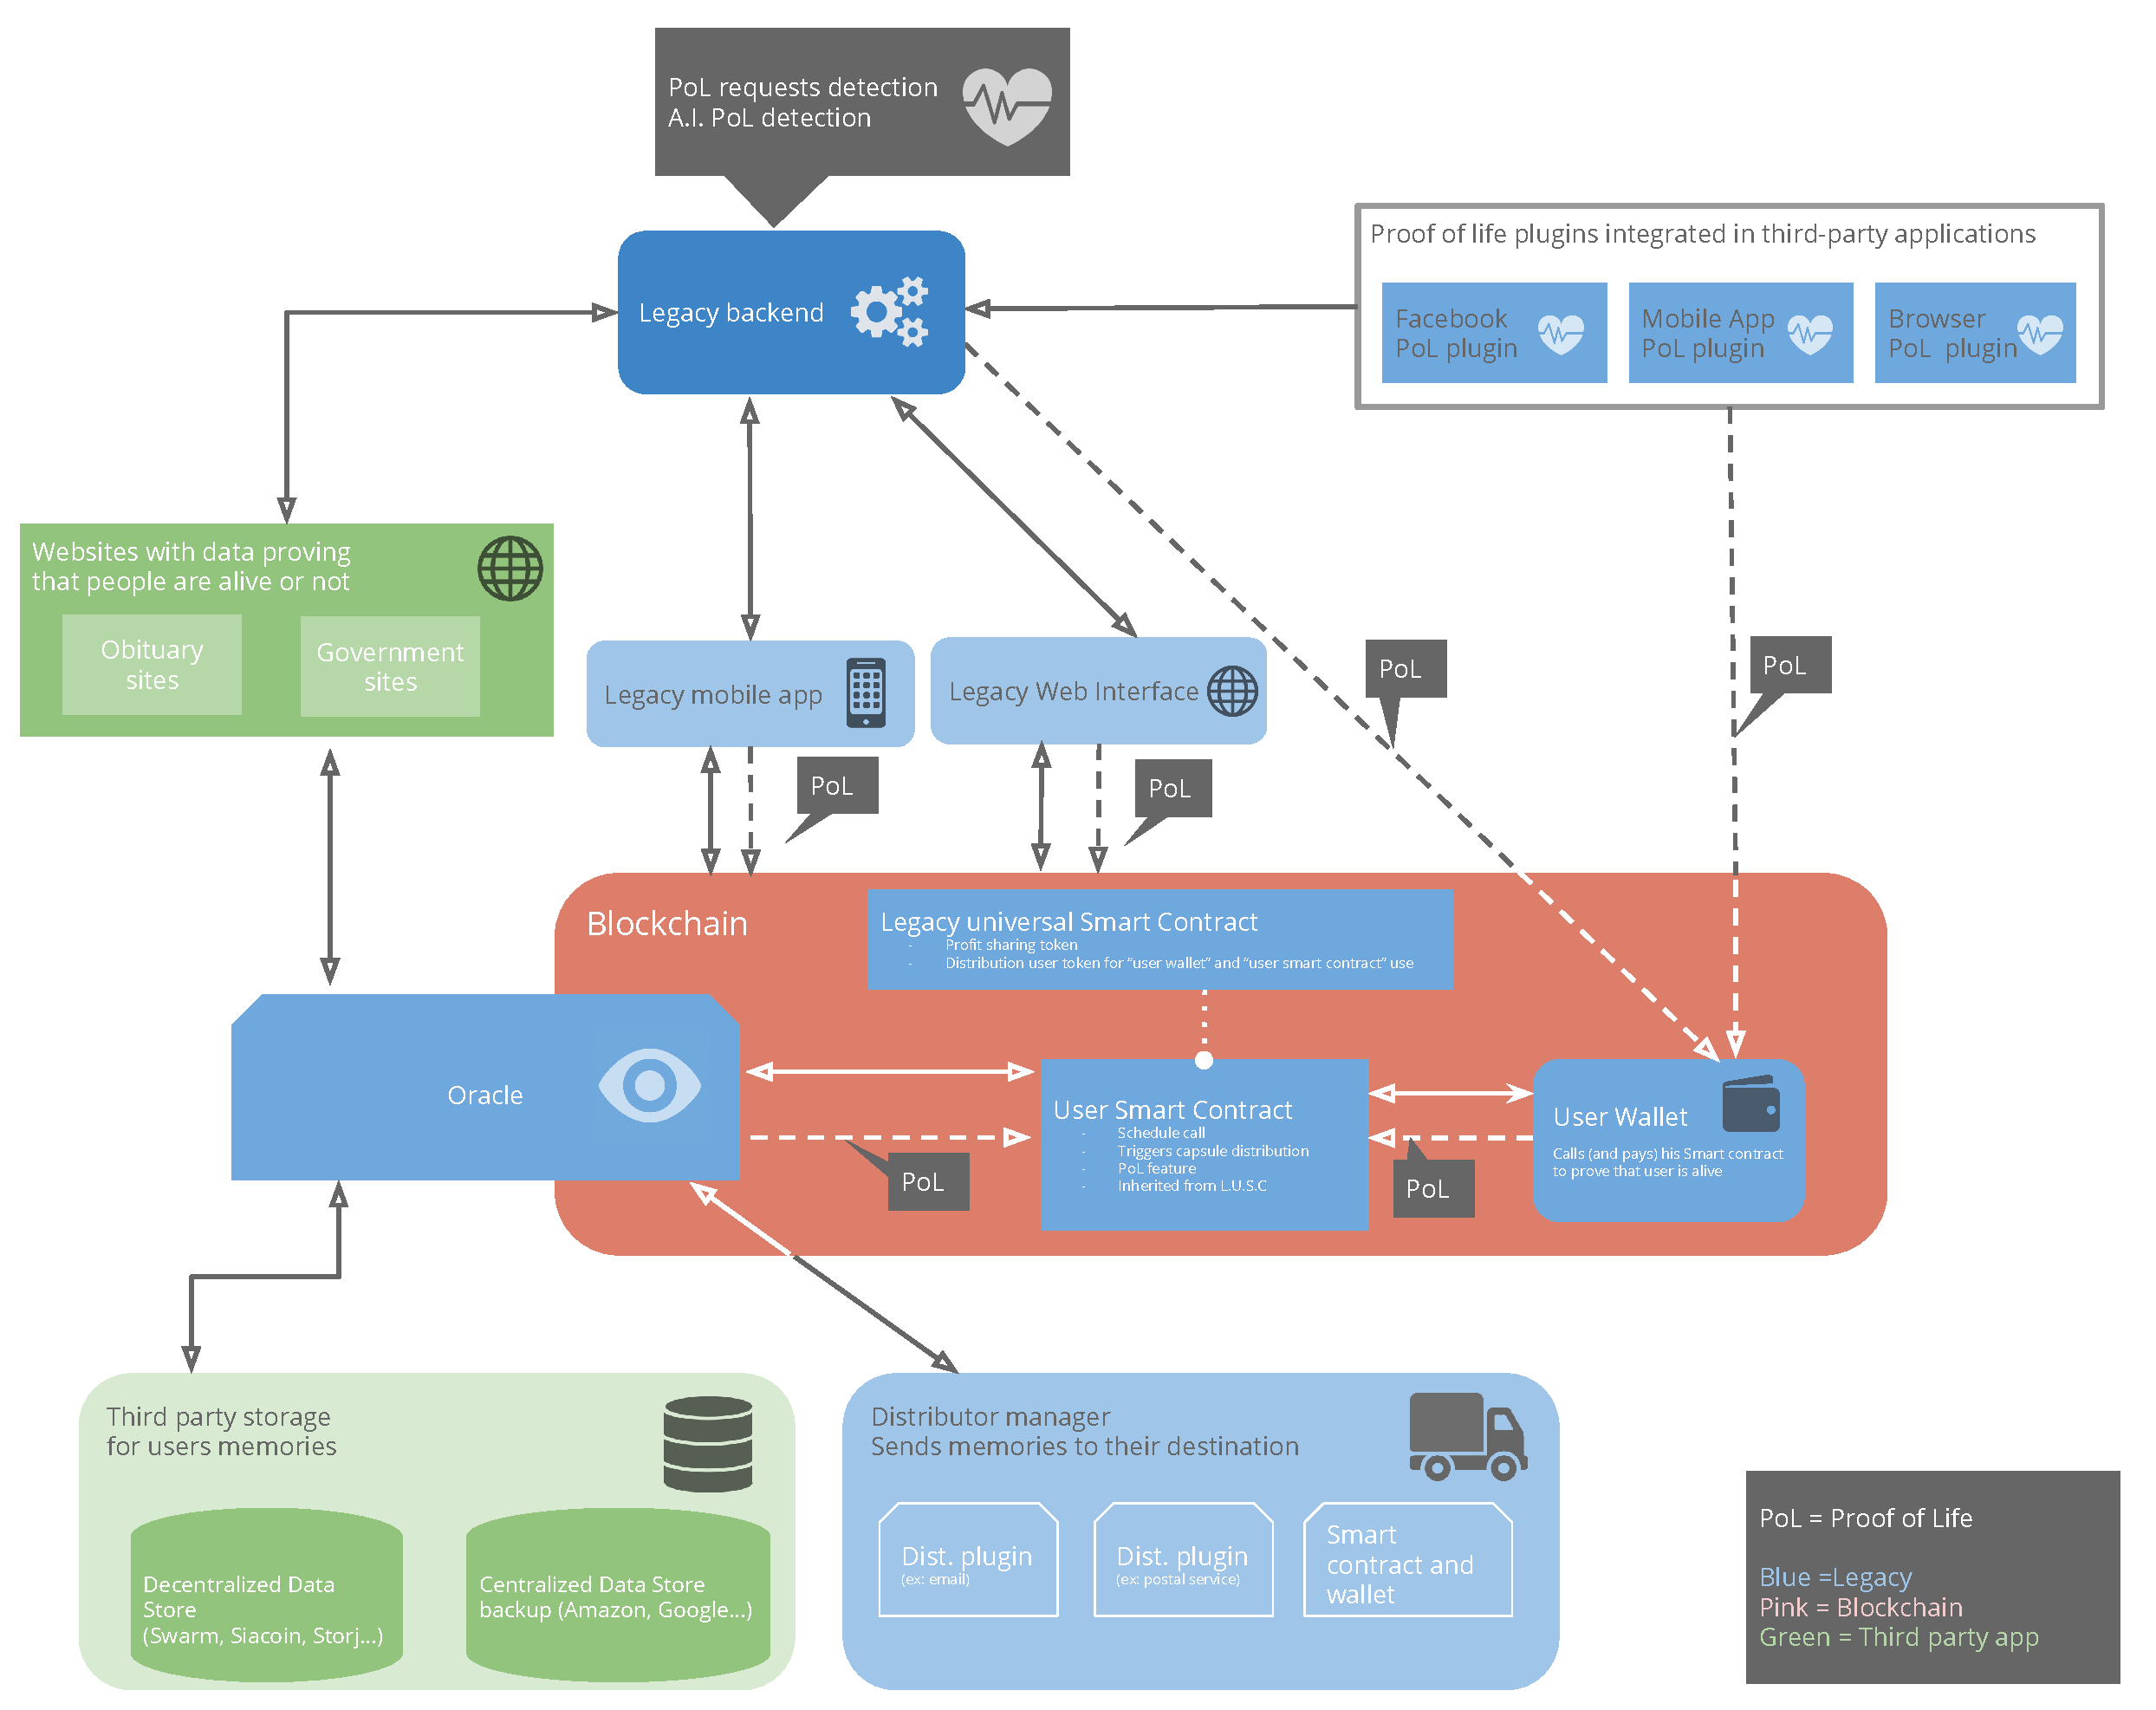
\includegraphics[scale=0.3]{fig/architecture_v02_hybrid}
  \caption{Legacy Mémoires architecture.}
  \label{fig:leg_v1_arch}
\end{figure} 

% subsection legacy_v1_0_memoirs_a_hybrid_architecture (end)

\section{Legacy v2.0 (Heritage): Towards a Fully Decentralized Architecture} % (fold)
\label{sec:legacy_v2_0_heritage_towards_a_fully_decentralized_architecture}
Legacy v2.0 Heritage will be Legacy’s second stable release. It main differences with respect to Legacy Memoirs are in the underlying architecture. This version intends to take maximum advantage of blockchain features offering, in particular, on-chain storage services and improved privacy. 
% TO-DO
Release of this version is estimated for 2020, though it is subject to the technological advances in the blockchain ecosystem.
% subsection legacy_v2_0_heritage_towards_a_fully_decentralized_architecture (end)

% chapter architecture (end)
\chapter{The Legacy Token} % (fold)
\label{cha:the_legacy_token}

The Legacy token, called LEG, will be created during a token sale event organized to fund the project. The token sale process will follow standard modalities established in the blockchain community. Once the token sale period is finished, no additional tokens will be generated. A maximum of 100.000.000 LEG can be created. 
Table \ref{table:ico_summary} provides some preliminary\footnote{The details regarding token supply distribution are subject to further changes as the exact crowdsale modality is not yet defined.} details regarding the token and its supply distribution. Additional details regarding the token sale process and how to participate in it will be provided in Legacy's official website \cite{Legacy}.

\begin{table}[h]
	\begin{center}		
		{\renewcommand{\arraystretch}{1.3}			
			\begin{tabular}{| l | p{5cm} | p{3.5cm}  |}	
		    \hline			    
		    	Total Supply		&  100 000 000 [LEG]  \\ \hline % TO-DO
		    	Auction Model       &  fixed-price auction\tablefootnote{To be confirmed.} \\ \hline														
				Percentage of supply available for crowdsale & 60\% \\ \hline
				Percentage of supply for Legacy founders     &  6\% \\ \hline
				Percentage of supply for Legacy Organization & 15\% \\ \hline
				Percentage of supply for advisors, partners and consultants & 12\% \\ \hline
				Percentage of supply for Legacy Foundation & 7\% \\	\hline	
			\end{tabular}				
		}
	\caption{Token sale summary.}
	\label{table:ico_summary}		
	\end{center}
\end{table}



The Legacy token serves three main purposes:

\begin{enumerate}
	\item It allows to create a shared economy on top of Legacy's platform. In this way, once Legacy is able to handle digital assets holding monetary value, experts and professionals such as lawyers, accountants or notaries may provide technical assistance to users managing complex holdings or in case specific legal requirements must be met according to local regulations related to property disposition through wills. In this context, the legacy token can be used to enable peer-to-peer transfer of value on the platform.
	\item In line with the previous idea, tokens can be used to implement a reward and incentive system allowing to encourage continuous platform development. Users may propose novel functionalities (for instant, a specific PoL plugin or a novel storage system) which can be implemented by developers in the community. Once a novel functionality is added to the platform, a fraction of the service fees are sent to its authors.
	This idea is further discussed in Section \ref{sub:a_reward_system_to_reinforce_long_term_service_availability}.
	\item Finally, LEG tokens can be used by users to gain access to commercial advantages. Paying for the service directly in LEG may give access to reduced service costs and other types of commercial incentives. This is a standard strategy to encourage token demand and also allows to implement fiscal policies regarding the token economics \cite{Sehra2017}.

\end{enumerate}

% TO-DO: add diagram
A simplified diagram showing how the token is employed in the application is presented in Appendix \ref{cha:economic_flow_model} (note that this simplified model does not include the use of the token for peer-to-peer transfer of value).

% \section{Legacy's Economic Model} % (fold)
% \label{sec:legacy_s_economic_model}
% TO-DO
% section legacy_s_economic_model (end)

% chapter the_legacy_token (end)
%\chapter{Roadmap} % (fold)
\label{cha:roadmap}

\begin{itemize}
	\item \textbf{Q1 2018: Legacy Alpha}. Runs on Testnet. Provides basic functionalities. Proof of life scheduled through smart contract. Local or centralised file storage.
	\item \textbf{Q2 2018: Legacy Beta}. Starting audit period. Continuously adding new plugins for PoL.
	\item \textbf{Q4 2018: Legacy v1.0/Mémoires}. Hybrid architecture. Keys and file storage using decentralised third-party service. PoL from decentralized smart contract and using Legacy's web services. Min. cap required of 3–4M USD.
	\item \textbf{Q3 2020: Legacy v2.0/Heritage}. Fully decentralized architecture. Encrypted, blockchain-based data storage. PoL fully managed by smart contract.
	\item \textbf{Future Releases}. Fully blockchain/tech agnostic. This version has no date specified in development, it depends highly on amount raised, evolution of blockchain tech and legal aspects.
\end{itemize}


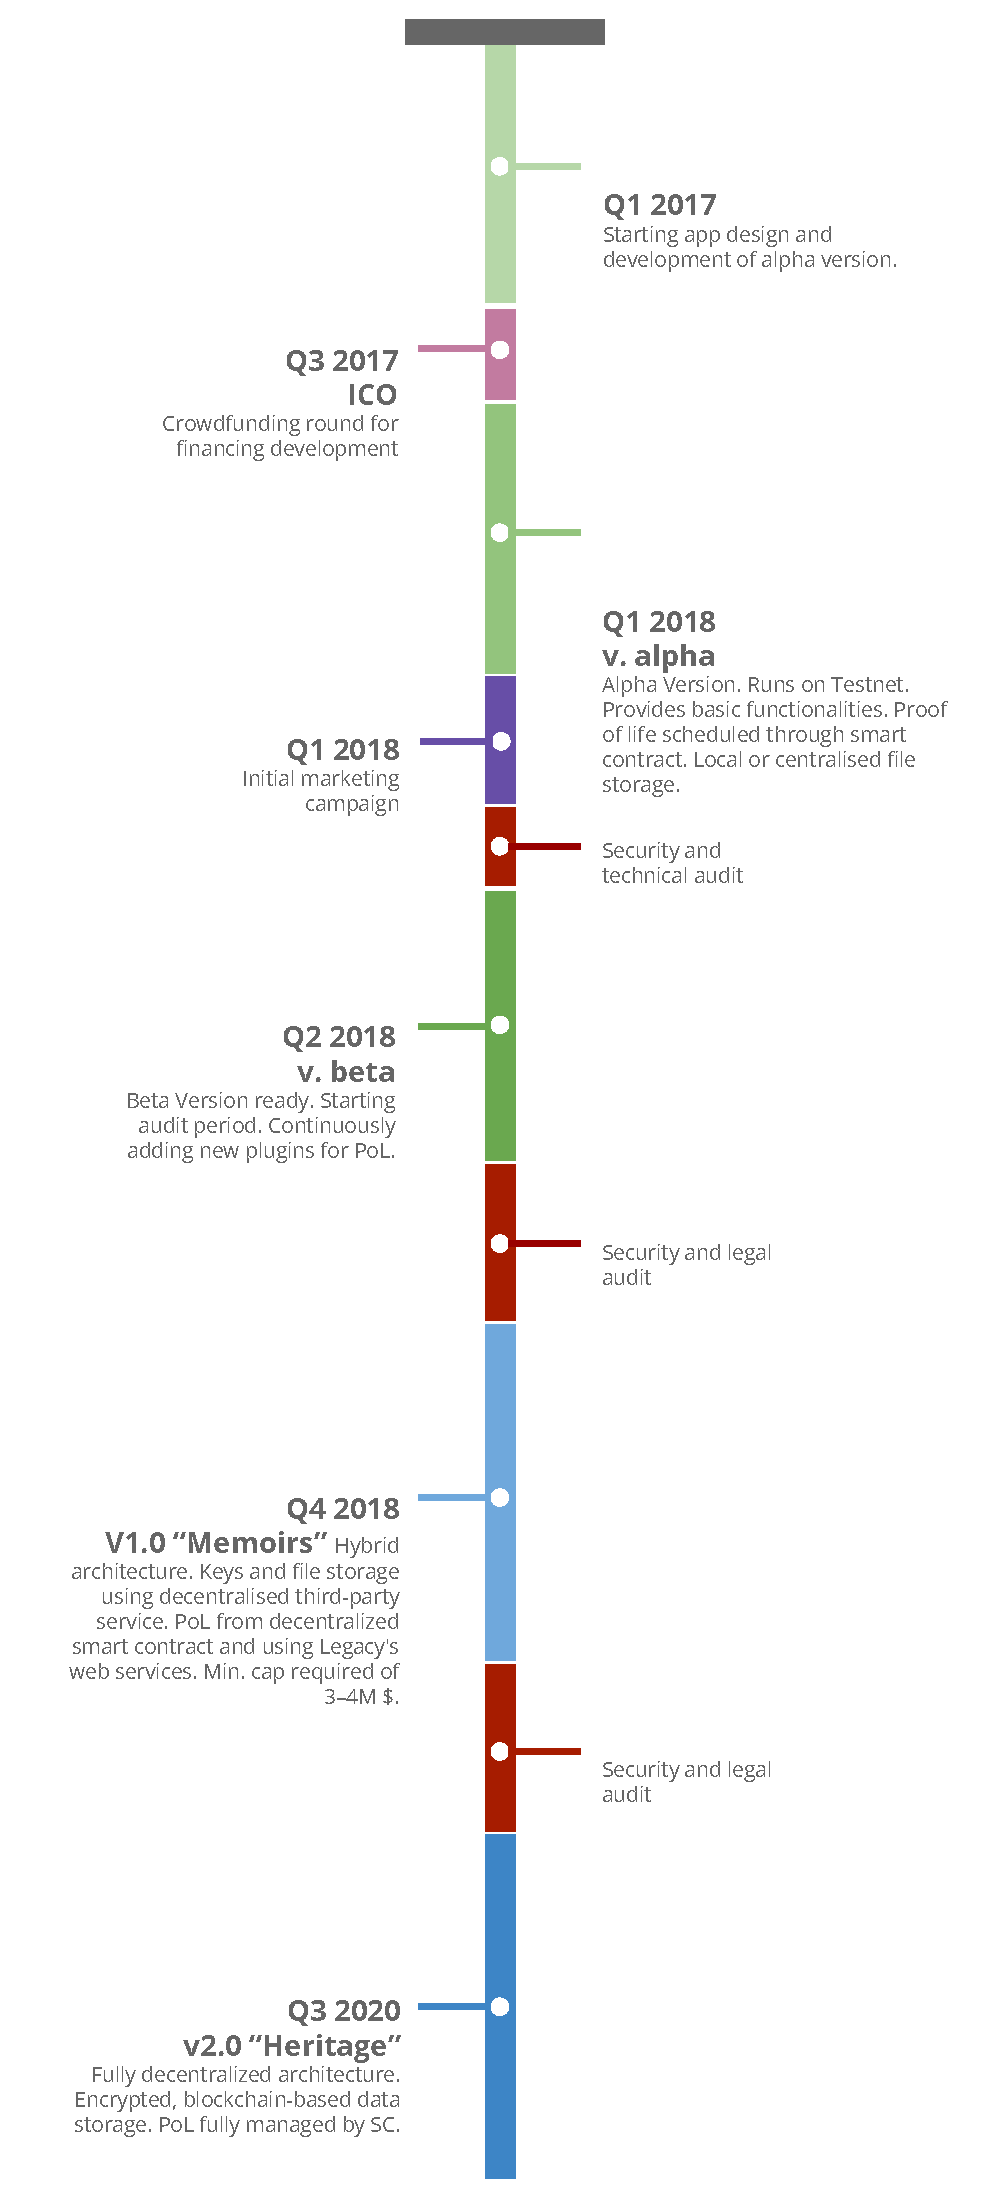
\includegraphics[scale=0.6]{fig/roadmap_vertical.pdf}

\section{Activities \& Resources} % (fold)
\label{sec:activities_resources}
The Legacy Team will work in two phases: the first one, starting immediately after the ICO, will be the implementation of our proposed solution. In the second phase, marketing, communication, legal, and customer service specialists will be added to the team to grow the user base, while production continues.

\subsubsection*{Phase 1: Production} % (fold)
\label{ssub:phase_1_production}
Using ICO funding, the first phase of the project is to publish the first stable release of Legacy I (Memoirs). Priority will be given to the development team, and marketing will be slowly ramped up as the release nears.

Key resources: blockchain specialists, developers, ICO funding.

% subsubsection phase_1_production (end)

\subsubsection{Phase 2: Marketing \& continued production} % (fold)
\label{ssub:phase_2_marketing_continued_production}
Once Legacy is operational, convincing customers outside the blockchain crowd will become the new priority.

Key resources: marketing and legal specialists in addition to core team.

% subsubsection phase_2_marketing_continued_production (end)

% section activities_resources (end)

% chapter roadmap (end)
\chapter{Legal Considerations} % (fold)
\label{cha:legal_considerations}

\textit{[WIP]}
\\
It is clear that Legacy may involve several legal issues that go beyond the team expertise---at least in its current form. Some legal issues identified so far include:

\begin{itemize}
	\item \textit{[list possible issues]}
\end{itemize}


% ---------------------------------------------------------------------------------------------------------------- %
% Foundation
% ---------------------------------------------------------------------------------------------------------------- %
\section{The Legacy Foundation} % (fold)
\label{sec:the_legacy_foundation}

Even if all technical aspects are working perfectly, finding people to deliver memories entrusted to Legacy may be difficult. Recipients may move, change their phone numbers, email addresses, etc. These edge cases can be handled by a separate, non-profit foundation.
The foundation will take care of correctly transmitting user’s assets if and only if purely automated means fail. 
The second mission of the foundation will be to advocate for change in the legislative process of transmitting properties.
In addition, the foundation may also run storage nodes to improve service reliability.

In order to ensure correct operation, the Legacy Foundation will receive a percentage of the service operation fees, which will be automatically transferred from user’s smart contracts once the service is paid.


% section the_legacy_foundation (end)

% chapter legal_consideration (end)
%\chapter{Crowdfunding} % (fold)
\label{cha:crowdfunding}

The Legacy project will be funded through a token crowdsale. The Legacy token, called LEG, serves two main purposes: it is used internally to execute the smart contracts residing in the Ethereum blockchain; and it allows for profit sharing among its holders.  Appendix \ref{} The token sale process follows standard modalities established in the blockchain ecosystem. In addition, it is in the Legacy spirit to provide additional investor protection by following recent recommendations given by the community. In particular, a minimum cap (or soft cap) target has been established, meaning that investor’s contributions will be refunded in case this target is not reached. Table \ref{table:ico_summary} summarizes the main aspects of the crowdsale.

\begin{table}[h]
	\begin{center}
		% \resizebox{\columnwidth}{!}
		% {
			\small
			\begin{tabular}{| l | p{5cm} | p{3cm}  |}	
		    \hline	
		    %\textbf{RA scheme} 	& \textbf{Peak  $T_{max}$ [b/s/Hz]}	& 	\textbf{$T$ at target $P_e\leq10^{-3}$ [b/s/Hz]}  &  \textbf{Observations}  \\ \hline    
		    	Total Supply		&  100 000 000 [LEG]  \\ \hline
		    	Auction Model       &  Ascending-price auction \\ \hline
				Starting date       &  2017/09/15\footnote{Not confirmed.} \\ \hline
				Ending date         &  starting date + 4 weeks or when the max cap is reached \\ \hline
				Maximum cap         &  100 000 [ETH] \\ \hline
				Soft cap            &  10 000 [ETH] \\ \hline
				Percentage of supply available for investors & 75\% \\ \hline
				Percentage of supply for Legacy founders     &  6\% \\ \hline
				Percentage of supply for Legacy Organization & 15\% \\ \hline
				Percentage of supply for advisors, partners and consultants & 4\% \\
			\hline	
			\end{tabular}				
		% }
	\caption{Token sale summary.}
	\label{table:ico_summary}		
	\end{center}
\end{table}


LEG tokens will be created dynamically during the token sale period. Once this period is finished, no additional tokens will be generated. A maximum of 100.000.000 LEG will be created. The token sale period finishes automatically at the predefined ending date or when the maximum cap is reached, whichever comes first.

The token sale follows a linear ascending-price model, according to Table \ref{table:ico_summary}.

\begin{table}[h]
	\begin{center}
		% \resizebox{\columnwidth}{!}
		% {
			\small
			\begin{tabular}{| l | p{5cm} | p{3cm}  |}	
		    \hline	
		    %\textbf{RA scheme} 	& \textbf{Peak  $T_{max}$ [b/s/Hz]}	& 	\textbf{$T$ at target $P_e\leq10^{-3}$ [b/s/Hz]}  &  \textbf{Observations}  \\ \hline    
		    	Phase I		&  1 ETH = 1000 LEG  \\ \hline
		    	Phase II		&  1 ETH = 900 LEG  \\ \hline
		    	Phase III	&  1 ETH = 800 LEG  \\ \hline
		    	Phase IV		&  1 ETH = 700 LEG  \\		    	
			\hline	
			\end{tabular}				
		% }
	\caption{Token price.}
	\label{table:ico_summary}		
	\end{center}
\end{table}

Detailed instructions for contributing to the crowdfunding campaign will be published on the official Legacy website several days before the starting date.  
Crowdsale Objectives

% Include diagram showing functionalities vs level of funding reached.
% What can we provide with minimum fund? with 2x min fund? with maximum fund?

% chapter crowdfunding (end)



%\chapter{The Team} % (fold)
\label{cha:the_team}

As shown throughout this paper, the Legacy Project involves several technical challenges. 
Legacy will not be an easy task, creating it will take time and will require a strong team capable of developing a product that will be used by our customers.

The Legacy team is composed by entrepreneurs and engineers with proven track records in creating, running and managing startup companies. Most of them participated in startup accelerator programs and founded companies which have delivered valuable products.


\textbf{Felipe Faraggi}
\textbf{CEO}
linkedin
Solidity Documentation Translator / Entrepreneur / Python Developer
Previous projects: etheresante.com, willty.com, yagan.io, lavillenue.fr
Master in Urban Architecture, Universidad Diego Portales, Santiago, Chile

\textbf{Vicente Almonacid}
\textbf{R\&D}
linkedin
PhD Candidate / Network & Communications Protocols / Satellite and IoT/M2M
MEng. TELECOM Bretagne, Brest, France; BSc in Telematics Engineering, USM, Valparaíso, Chile.

\textbf{Guillaume Figielski}
\textbf{Architecture}
linkedin
CS Engineer / Solidity Specialist / VR Professional
Previous projects: girosense.com
French Engineer in Computer Science, 3IL (Engineer school), Limoges, France.
MS in Software Engineering, University of Quebec at Chicoutimi (UQAC), Chicoutimi, Canada. 

\textbf{Nicolas Michel}
\textbf{System Operations}
linkedin
CS Engineer / Blockchain Specialist / Legal Theory
Previous projects: unooc.fr, axonaut.com
MS in Software Engineering, University of Toulouse (Paul Sabatier), Toulouse, France.

\textbf{Nicolas Ricard}
\textbf{Lead Developer}
linkedin
CS Engineer / Web developer / Backend
Previous projects: unooc.fr, axonaut.com
MS in Software Engineering, University of Toulouse (Paul Sabatier), Toulouse, France.

\section{Transparency} % (fold)
\label{sec:transparency}
Ensuring transparent communication with the community is one of the top priorities of Legacy. The team is committed to actively provide updates and to quickly respond to feedback from investors, token holders and users.

Official communication channels will be listed on Legacy’s website.

KPI reports, as well as more detailed analysis will be periodically published on our website and transmitted to the mailing list.

% section transparency (end)

% chapter the_team (end)

% ---------------------- %
% Appendix
% ---------------------- %
%\appendix
\begin{appendices} % to use with \usepackage[titletoc]{appendix}
% ---------------------------------------------------------------------------------------------------------------- %
% Competitors
% ---------------------------------------------------------------------------------------------------------------- %
% \chapter{List of Potential Competitors} % (fold)
% \label{cha:list_of_potential_competitors}

% \begin{itemize}
% 	\item \url{Digipulse.io}
% 	\item \url{lastwill.io}
% 	\item \url{legacyvault.com}
% 	\item \url{loggacy.com} (closed down)
% 	\item \url{mymoriam.com}
% 	\item \url{knotify.me}
% 	\item \url{estatemap.com}
% 	\item \url{everplans.com}
% 	\item \url{afternote.com}
% 	\item \url{boxego.com}
% 	\item \url{chronicleoflife.com}
% 	\item \url{safebeyond.com}
% \end{itemize}
% chapter list_of_potential_competitors (end)

% ---------------------------------------------------------------------------------------------------------------- %
% Flow Chart
% ---------------------------------------------------------------------------------------------------------------- %
\chapter{Flow Chart} % (fold)
\label{cha:flow_chart}
\begin{figure}
	\centering
	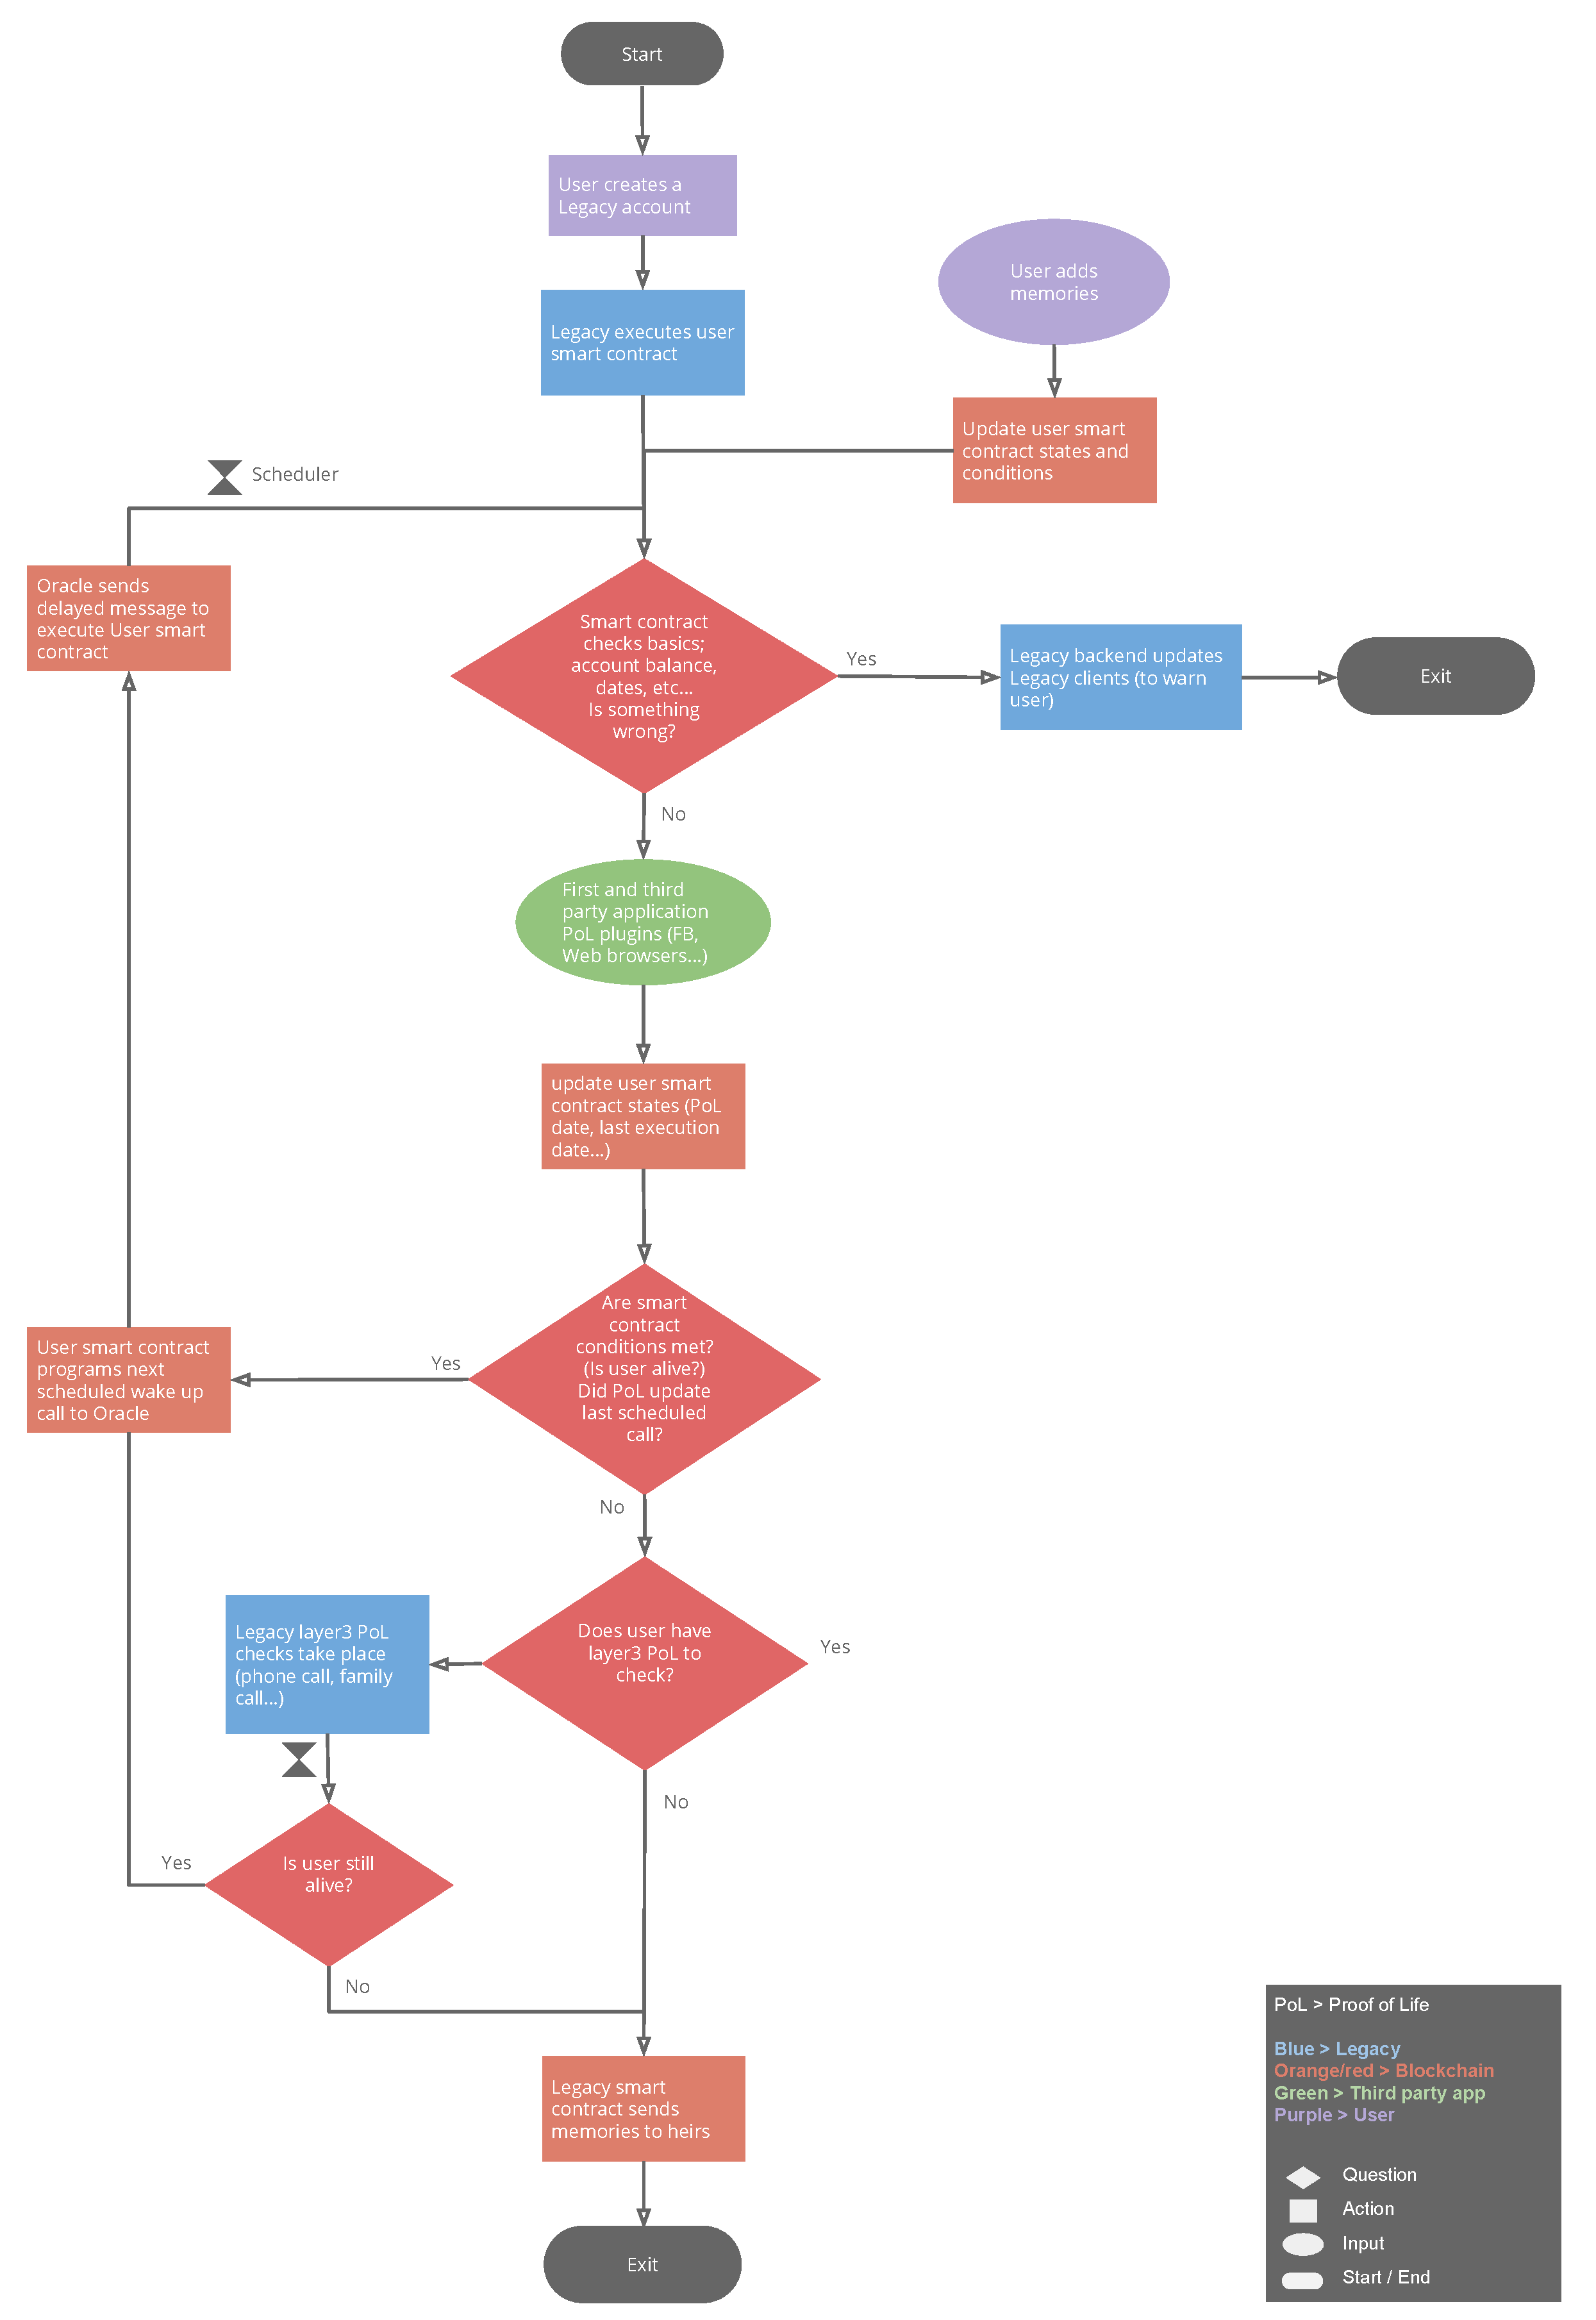
\includegraphics[scale=0.4]{fig/flow_chart_short_version.pdf}
	\caption{Application flow chart.}
	\label{fig:flow_chart}
\end{figure}
% chapter flow_chart (end)


% ---------------------------------------------------------------------------------------------------------------- %
% Economic Flow Model
% ---------------------------------------------------------------------------------------------------------------- %
\chapter{Economic Flow Model} % (fold)
\label{cha:economic_flow_model}
\begin{sidewaysfigure}
	\centering
	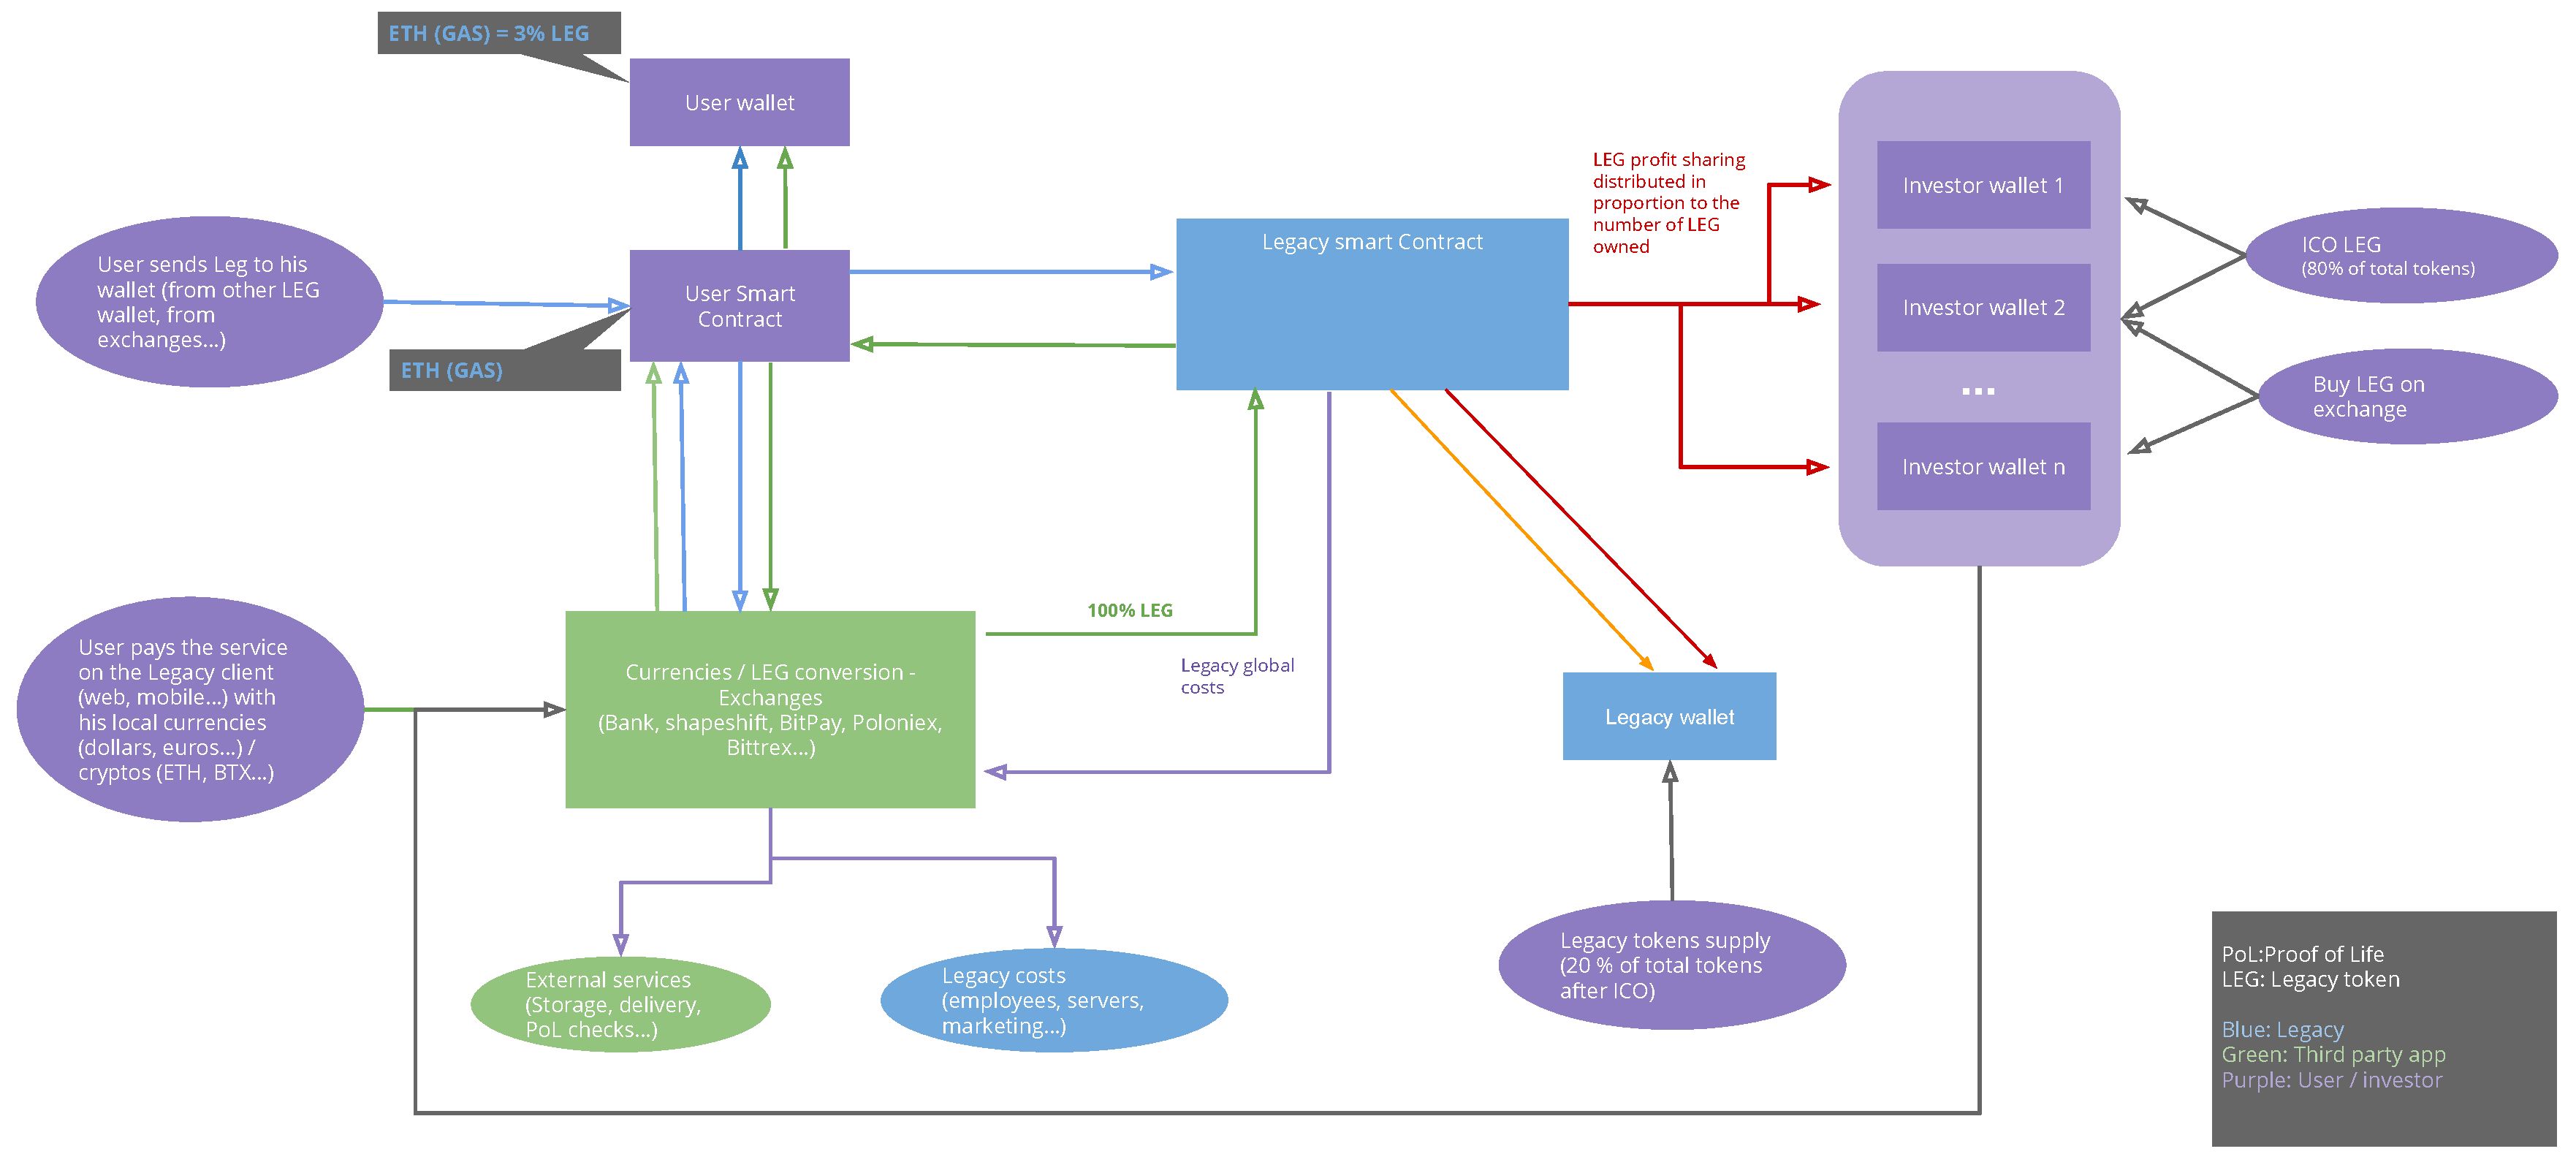
\includegraphics[scale=0.4]{fig/profit_sharing_model_v02.pdf}
	\caption{Legacy's economic flow model.}
	\label{fig:economic_flow}
\end{sidewaysfigure}
% chapter economic_flow_model (end)

\end{appendices}


% ---------------------- %
% Bibliography
% ---------------------- %
%
% 1. using natbib
%\bibliographystyle{plain}
%\bibliography{\bibpath/refs}
%
% 2. uing biblatex
\printbibliography

\end{document}}
